\documentclass[10pt,final,journal,twoside]{IEEEtran}
\usepackage{amsmath,amsfonts}
\usepackage{algorithmic}
\usepackage{array}
\usepackage{caption}
\usepackage[caption=false,font=normalsize,labelfont=sf,textfont=sf]{subfig}
\usepackage{textcomp}
\usepackage{stfloats}
\usepackage{url}
\usepackage{verbatim}
\usepackage{graphicx}
\hyphenation{op-tical net-works semi-conduc-tor IEEE-Xplore}
\def\BibTeX{{\rm B\kern-.05em{\sc i\kern-.025em b}\kern-.08em
    T\kern-.1667em\lower.7ex\hbox{E}\kern-.125emX}}
\usepackage{balance}
\usepackage{cite}
\usepackage[T1]{fontenc} % optional
\usepackage[cmintegrals]{newtxmath}
\usepackage{bm} % optional
\usepackage{physics}
\usepackage{makecell}
\usepackage{float}
\usepackage{placeins} % equivalent to add ``\FloatBarrier'' before each Section
% \usepackage{mathrsfs} % providing the command \mathscr{}
% It is strongly recommended to use hyperref, especially for the review version.
% hyperref with option pagebackref eases the reviewers' job.
% Please disable hyperref *only* if you encounter grave issues, e.g. with the
% file validation for the camera-ready version.
%
% If you comment hyperref and then uncomment it, you should delete
% ReviewTempalte.aux before re-running LaTeX.
% (Or just hit 'q' on the first LaTeX run, let it finish, and you
%  should be clear).
\usepackage[pagebackref=false,breaklinks,hidelinks]{hyperref}
% Support for easy cross-referencing
% \usepackage[capitalize]{cleveref}
% \usepackage{subfigure} %% NOT COMPATIBLE WITH <HYPERREF>!!! USE <SUBCAPTION> INSTEAD!!!

\setlength{\IEEEdlabelindent}{0pt}

\newtheorem{theorem}{Theorem}
\newtheorem{lemma}{Lemma}
\newtheorem{proposition}{Proposition}
\newtheorem{definition}{Definition}
\newtheorem{algorithm}{Algorithm}

\captionsetup[subfloat]{font=footnotesize,labelfont=rm,farskip=0pt}

\allowdisplaybreaks

\begin{document}
\bstctlcite{IEEEexample:BSTcontrol}
\title{Improving Synchronization Stability of VSC via Novel Anti-windup Augmented Phase-Locked Loop}
\author{Zhenke Zhang,~Yuanlong Li,~Fei Gao.
\thanks{This work was supported by the National Natural Science Foundation of China under Grant Nos. 62373249 and 62022055. Corresponding author
Y. Li}
\thanks{Email addresses:~JohnJackal@sjtu.edu.cn~(Zhenke Zhang),\\liyuanlong0301@sjtu.edu.cn~(Yuanlong Li).}}
\markboth{Journal of \LaTeX\ Class Files,~Vol.~18, No.~9, September~2020}
{Zhang,~\MakeLowercase{\textit{et al.}}:~Improving Synchronization Stability of VSC via Novel Anti-windup Augmented Phase-Locked Loop}
\maketitle

\begin{abstract}
It is challenging to guarantee the synchronization stability of grid-following VSC during severe ac-grid faults, due to the vulnerability of the commonly used synchronous reference frame phase-locked
loop (SRF-PLL) to grid voltage variation. Previous researches usually sacrifice the computation cost and latency for stability gains, as seen in methods like DDSRF-PLL. Attempts have also been made to introduce
artificial limiter and anti-windup mechanism to the SRF-PLL, but their effectiveness in improving stability has not yet been confirmed. In this paper, we propose a performance-activated anti-windup augmented PLL
in order to enlarge the long-term grid fault tolerance of grid-following VSC, hence improving the system synchronization stability. The phase difference between PCC and grid is taken as the performance
indicator, and is injected to the input of the artificial limiter to control the activation time of the anti-windup compensator. An iterative optimization algorithm is developed to determine the parameters
of the anti-windup compensator. Simulation results proved the effectiveness of the proposed PLL configuration.
% In the face of severe AC-grid faults, ensuring the stability of grid-following VSC synchronization poses a formidable challenge, persisting as an unresolved issue. This study introduces an innovative
% structure for PLL, bolstered by performance-driven anti-windup augmentation, aimed at enhancing synchronization stability in grid-following VSC systems under severe grid faults. To ascertain optimal
% parameters for the anti-windup compensator, an iterative optimization algorithm is devised. The simulation outcomes underscore the efficacy of the suggested PLL setup.
% Maintaining synchronization stability of grid-following VSC during severe ac-grid faults is a challenging task and remains an open problem. In this paper, we propose a novel performance-activated
% anti-windup augmented PLL structure in order to improve the synchronization stability of grid-following VSC against severe grid faults. An iterative optimization algorithm is formulated to determine
% the anti-windup compensator parameters. Simulation results demonstrated the effectiveness of the proposed PLL configuration.
\end{abstract}

\begin{IEEEkeywords}
Synchronization stability, long-term large disturbance, voltage-source converter (VSC), phase-locked loop (PLL), anti-windup, performance activation
\end{IEEEkeywords}

% Section I------------------------------------------------
\section{Introduction}\label{sec:intro}
\IEEEPARstart{D}{uring} the past few decades, an energy revolution has been gradually emerging all around the world. Renewable energy sources (RES) including photovoltaic power, wind power, hydropower, etc.,
have experienced a rapid development, prompting the advancement of power electronic grid interfaces like voltage-source converter (VSC)\cite{bose2017,mansoor2022}.
% To achieve the goal of "carbon peaking and carbon neutrality", China has vigorously developed renewable energy generation. Till now, the installed
% capacity of renewable energy sources such as photovoltaic and wind power of China ranks first in the world, making China the largest renewable energy country globally. By the end of 2022, the newly
% installed capacity of wind power and photovoltaic power nationwide reached 125 million kW, and that of all renewable energy sources reached 152 million kW, representing 76.2\% of the
% country's total newly added power generation capacity; the total installed capacity of renewable energy reached 1.213 billion kilowatts, accounting for 47.3\% of the total power generation
% capacity of China\cite{credr2022,rced2023,rcepd2023}.% The installed capacity of renewable energy is close to half of the total installed capacity, indicating a trend of replacing traditional thermal power as the mainstay of the power grid.
%\IEEEPARstart{O}{ver} the last few decades, the penetration of renewable energy source (RES) is continuously increasing due to its environmental friendliness and energy saving,
% which promotes the development of power electronic devices like voltage-source converter (VSC)\cite{bose2017,mansoor2022}.
% Typically, VSC is employed as the grid interface of distributed RESs\cite{mansoor2022,hu2019}.

Depending on the adopted control strategy, VSC can be divided into two categories: grid-following and grid-forming, with the former being the current mainstream\cite{pattabiraman2018}. Typically,
grid-following VSC depends on phase-locked loop (PLL) to keep synchronization with grid. When grid short-circuit faults occurs, the point of common coupling voltage would drop to a lower
value\cite{bookkundur1994}, causing the short circuit ratio at PCC to decrease, thereby weakening the connection between the RES and grid\cite{harnefors2007,zhang2011}. As a consequence, the synchronization
stability issue would arise when grid faults occur\cite{ma2018,he2021}.

Most of the previous researches focus on transient stability, as grid faults are assumed to be removed within a short time by the relay protection devices. However, the fault clearance takes time,
typically ranging from several hundred ms to several seconds, not to mention the possibility of relay protection failure. Thereby, the long-term fault voltage dip tolerance (FVDT) should be a critical
stability index of the VSC. Notice that the PCC voltage is the input of PLL, while the PLL dynamics determines the currents injected to
the grid from the grid-following VSC, which will affect the PCC voltage in turn\cite{dong2015}. Therefore, adjusting the current injected to ac-grid and modifying the PLL configuration are two feasible
approaches to enhance the synchronization stability of VSC.

The first approach, known as current injection strategy, can provide enough line current to maintain the PCC voltage, hence diminishing the affect of fault voltage dip.
An adaptive switching current injection strategy relying on grid impedance angle is introdeced in~\cite{ma2018}. However, it is nearly impossible for the local control terminal to know the grid
impedance angle, making the strategy impractical. Another strategy proposed in~\cite{geng2018} uses the disparity between the PLL-detected frequency and the grid's nominal frequency to
compensate the active current output of VSC, yet compromising the reactive current capability and requiring an additional STATCOM to supply extra reactive current, thereby reducing the system reliability
and increasing the cost.

In terms of PLL configuration modifying, there are numerous possibilities. In \cite{wu2020},
an adaptive PLL switching between SRF-PLL and first-order PLL is proposed, yet the switching threshold highly depends on the severity of the fault, and the steady-state error problem
also arises when the first-order PLL is activated. In~\cite{tang2023}, an artificial limiter is inserted at the output of the PI controller in SRF-PLL, forming a constrained PLL (CPLL), while
the ``windup'' problem caused by the limiter is not discussed, which would definitely degrade the system stability\cite{lozier1956,stein2003,bookofzac}. Another research force incorporated
the artificial limiter and some obsolete anti-windup compensators into the SRF-PLL\cite{chen2023}, finding that the limiter would damage the system transient stability, while the VSC with a back-calculation
anti-windup augmented PLL, which is equivalent to a static anti-windup augmented PLL (SAWAPLL), shows the largest FVDT among all the other anti-windup augmented PLLs and the original SRF-PLL.
Nevertheless, neither~\cite{chen2023} nor~\cite{tang2023} has considered the long-term FVDT.

In this paper, we apply the performance-activation mechanism for anti-windup compensators proposed in~\cite{lai2024} to the SAWAPLL, to improve the long-term FVDT of
the grid-following VSC. The rest of the paper is organized as follows. In~\autoref*{sec:impact}, the model of SRF-PLL is established, the impact of grid voltage fault on the synchronization stability
of the grid-following VSC is analyzed, and the long-term FVDT of CPLL and SAWAPLL is tested via simulation. In~\autoref*{sec:paawapll}, the model of performance-activated anti-windup augmented PLL
(PAAWAPLL) is established, and an anti-windup synthesis algorithm is developed. In~\autoref*{sec:valid}, the effectiveness of the proposed PLL in improving synchronization stability of grid-following VSC is
evaluated by simulation in two different scenarios. Finally, conclusions are drawn in~\autoref*{sec:conclusion}.\\
{\bf Notation.} For a square matrix A, $\textrm{He}(A)=A+A^T$. For any two integers $j_1<j_2$, $I[j_1,j_2]:=\{j_1,j_1+1,\ldots,j_2\}$.
% \clearpage

% Section II-------------------------------------------------
\section{Impact of Grid Faults on Synchronization Stability}\label{sec:impact}
\subsection{System Configuration}\label{subsec:config}
\begin{figure}[!t]
\centering
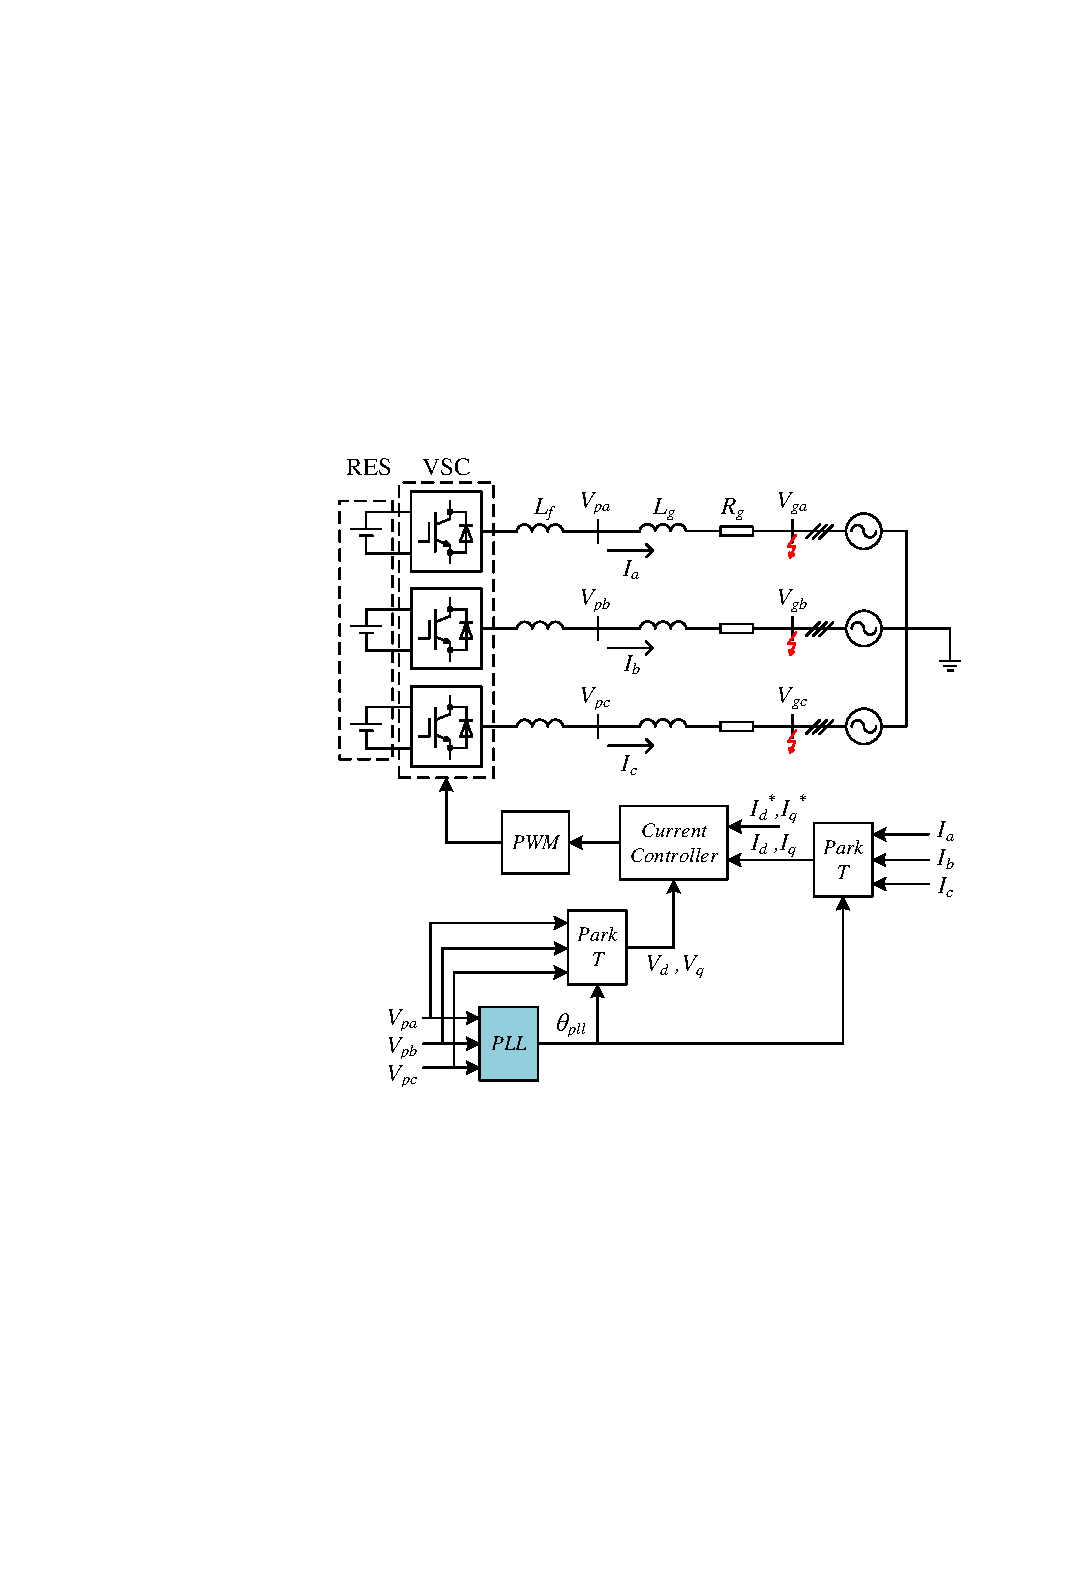
\includegraphics[width=1.0\linewidth]{../Diagrams/grid-connected_VSC.pdf}
\caption{Configuration of a simplified grid-following VSC system}
\label{fig_vsc}
\end{figure}

\figurename~\ref{fig_vsc} presents the configuration of a simplified grid-connected RES-VSC system, in which the transformers are omitted. The circuit parameters are presumed to be balanced in three phases.
The PCC voltages $V_p$ can be modelled by the grid voltage $V_{gx}$, line current $I_x$, and impedance $R_g+\omega_pL_g$ in the following phasor form,
\begin{equation}\label{circuitEq}
\bm{V}_{px}=\bm{V}_{gx}+R_g\bm{I}_x+j\omega_pL_g\bm{I}_x,
\end{equation}
% where $x$ denotes one of the three phases $A,\;B,\;C$.
where $x\in\{A,B,C\}$ denotes the phase, and $\omega_p$ denotes the grid angular frequency. Applying Park's transformation to (\ref{circuitEq}), we get the synchronous reference frame form,
\begin{equation}\label{circuitdqEq1}
\begin{cases}
    V_{pd}=V_g\cos\left(\theta_g-\theta_p\right)+R_gI_d-\omega_pL_gI_q\\
    V_{pq}=V_g\sin\left(\theta_g-\theta_p\right)+R_gI_q+\omega_pL_gI_d
\end{cases}
\end{equation}\par
Usually, the bandwidth of the current controller is much greater than that of the PLL, with the former being greater than $100Hz$\cite{morris2021} while the latter being about $10Hz$\cite{hu2017}.
This allows us to disregrad the transient behavior of currents when studying the synchronization stability of the system. Besides, $\theta_p,\omega_p$ should be replaced by the output of PLL
$\theta_{pll},\omega_{pll}$, and since $\theta_g$ is not accessible, we substitute it with $\theta_{gn}=\int_t\omega_{gn}\dd t$ without loss of generality. Define $\delta=\theta_{gn}-\theta_{pll}$
as the phase difference. Then we have the following circuit model in synchronous reference frame,
% In most cases, the bandwidth of the VSC current controller is greater than $100Hz$\cite{morris2021}, which is over 10 times higher than that of the PLL, with the latter being around $10Hz$\cite{hu2017}.
% This indicates that the current response of the VSC is much faster than the PLL dynamics, enabling us to neglect the current dynamics in the study of transient stability. Besides, $\omega_{g}$ and $\omega_{p}$
% should be replaced by their accessible counterparts, namely $\omega_{gn}$ and $\omega_{pll}$. The modified dq decoupled circuit model can be obtained as follows.
\begin{equation}\label{circuitdqEq2}
\begin{cases}
    V_{pd}=V_g\cos\delta+R_gI_d^*-\omega_{pll}L_gI_q^*,\\
    V_{pq}=-V_g\sin\delta+R_gI_q^*+\omega_{pll}L_gI_d^*,
\end{cases}
\end{equation}
\begin{figure}[!t]
\centering
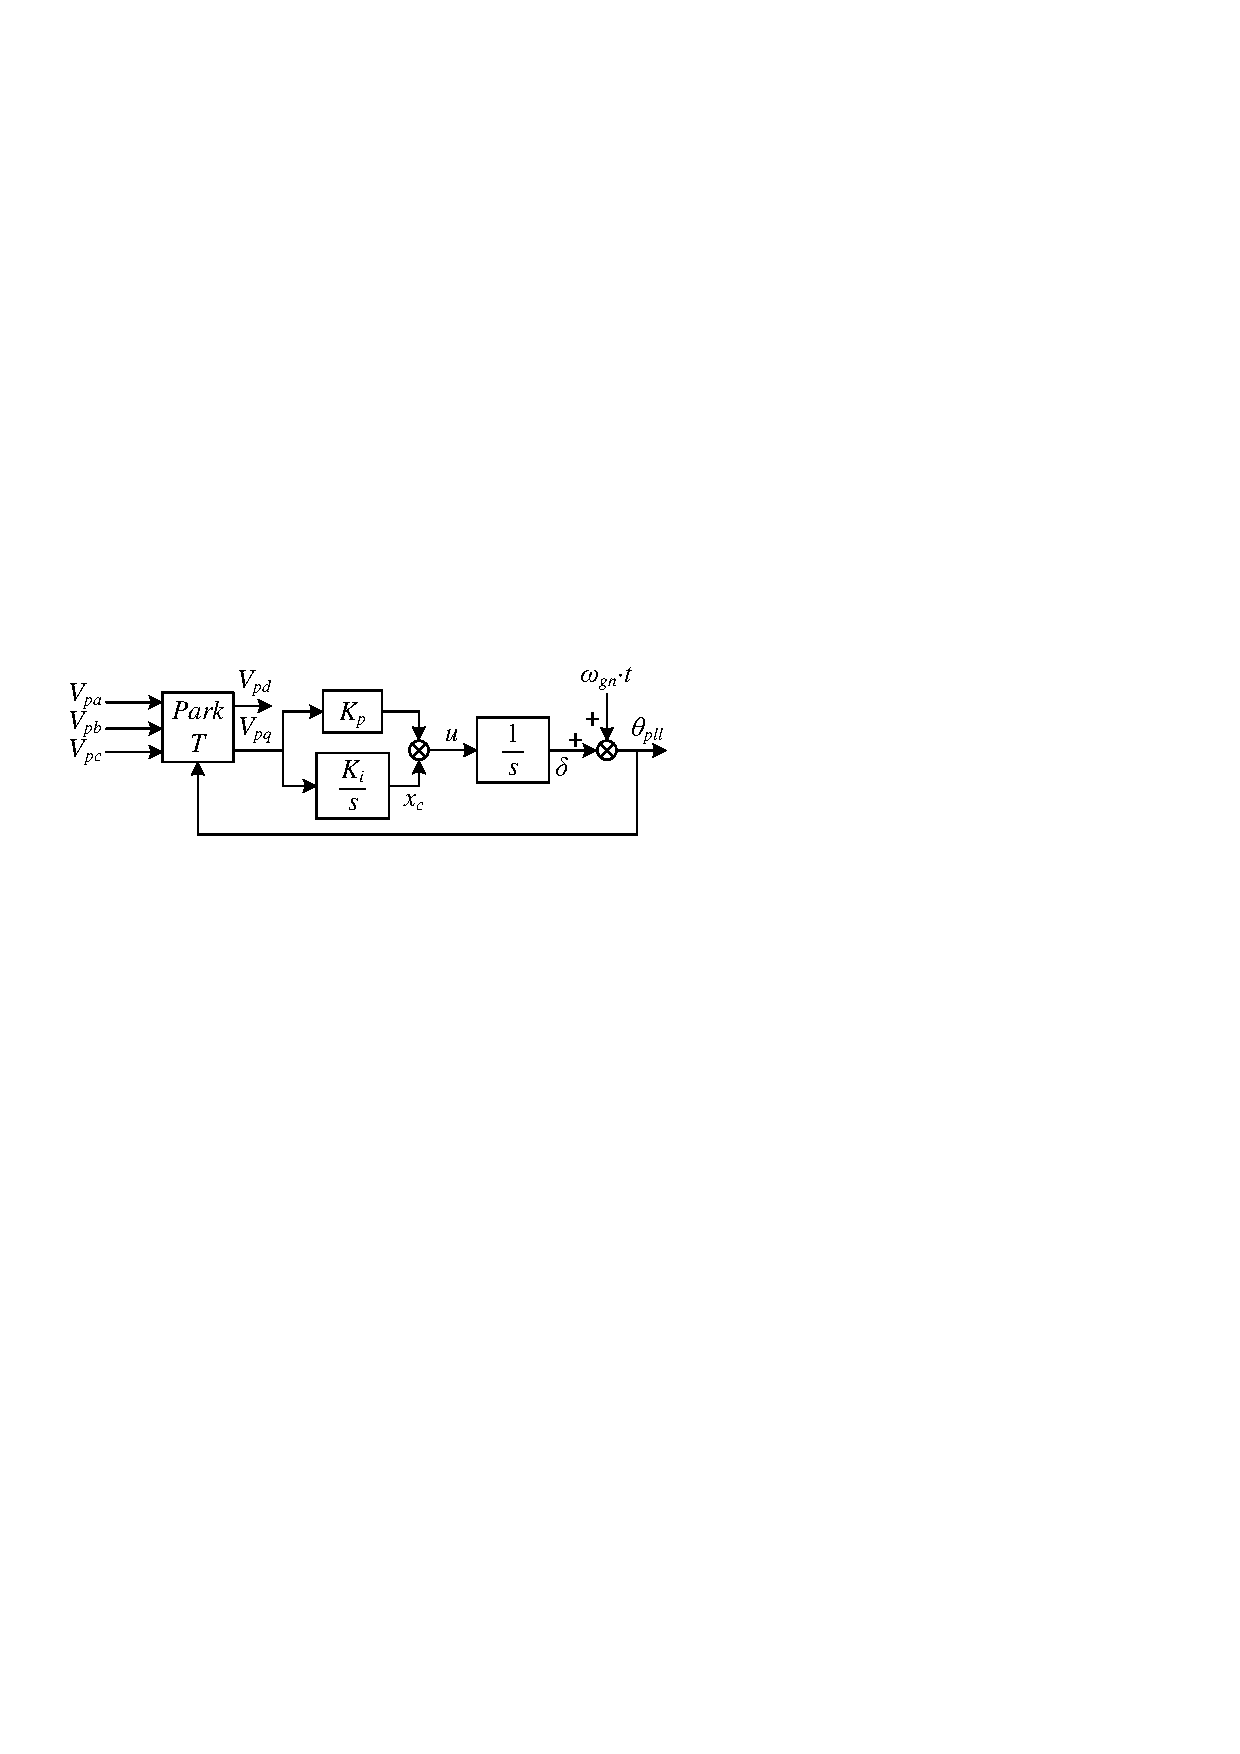
\includegraphics[width=.9\linewidth]{../Diagrams/PLL.pdf}
\caption{Diagram of SRF-PLL}
\label{fig_pll}
\end{figure}
where $I_d^*$ and $I_q^*$ are current references.\par
\figurename~\ref{fig_pll} shows the configuration of the original SRF-PLL. Denote $\delta_{ss}$ as the steady-state value of $\delta$. From (\ref{circuitdqEq2}), we have
\begin{equation}\label{dss}\delta_{ss}=\asin\left(\dfrac{R_gI_q^*+\omega_{gn}L_gI_d^*}{V_g}\right).\end{equation}

Denote $u$ as the PI controller output in PLL. Let $x_p=\delta-\delta_{ss}$ and $x_c=\int_tK_iV_{pq}$. Then the model of SRF-PLL is shown as follows
\begin{equation}\label{unPLL}
\left\{\begin{aligned}
    x_p=&\;u,\\
    x_c=&\;K_i\left(-V_g\sin\left(x_p+\delta_{ss}\right)+R_gI_q^*+\omega_{pll}L_gI_d^*\right),\\
    u=&\;x_c+K_p\left(-V_g\sin\left(x_p+\delta_{ss}\right)+R_gI_q^*+\omega_{pll}L_gI_d^*\right),\\
    \omega_{pll}=&\;u+\omega_{gn}.
\end{aligned}\right.
\end{equation}

Since the PLL model is nonlinear, we design the PI parameters of PLL based on the linearized model. In~\cite{bookofteodo}, the small signal model of SRF-PLL is discussed, with damping ratio $\zeta$ and settling time $t_s$ being
\begin{align}\label{PLLparam}
    \zeta&=\dfrac{K_p}{2}\sqrt{\dfrac{V_g}{2K_i}},\\
    t_s&=\dfrac{18.4}{K_pV_s}.
\end{align}
\begin{figure*}[!t]
\centering
\subfloat[][]{
\includegraphics[width=.5\linewidth]{../Diagrams/simulation_results_j/LIMIT.pdf}}
\subfloat[][]{
\includegraphics[width=.5\linewidth]{../Diagrams/simulation_results_j/LIMIT2.pdf}}
\caption{Simulation result of VSCs with SRF-PLL, CPLL, and SAWAPLL, in the HV scenario. The fault voltage dip magnitude is $-66\sqrt{2}kV$ in (a) and $-70\sqrt{2}kV$ in (b).}
\label{fig_limit}
\end{figure*}
The PI parameters of PLL can be determined by specifying the performance indices $\zeta$ and $t_s$. Both simulation and experiments in~\cite{wu2018} demonstrated the effectiveness of the design method.
\begin{figure*}[!b]
\centering
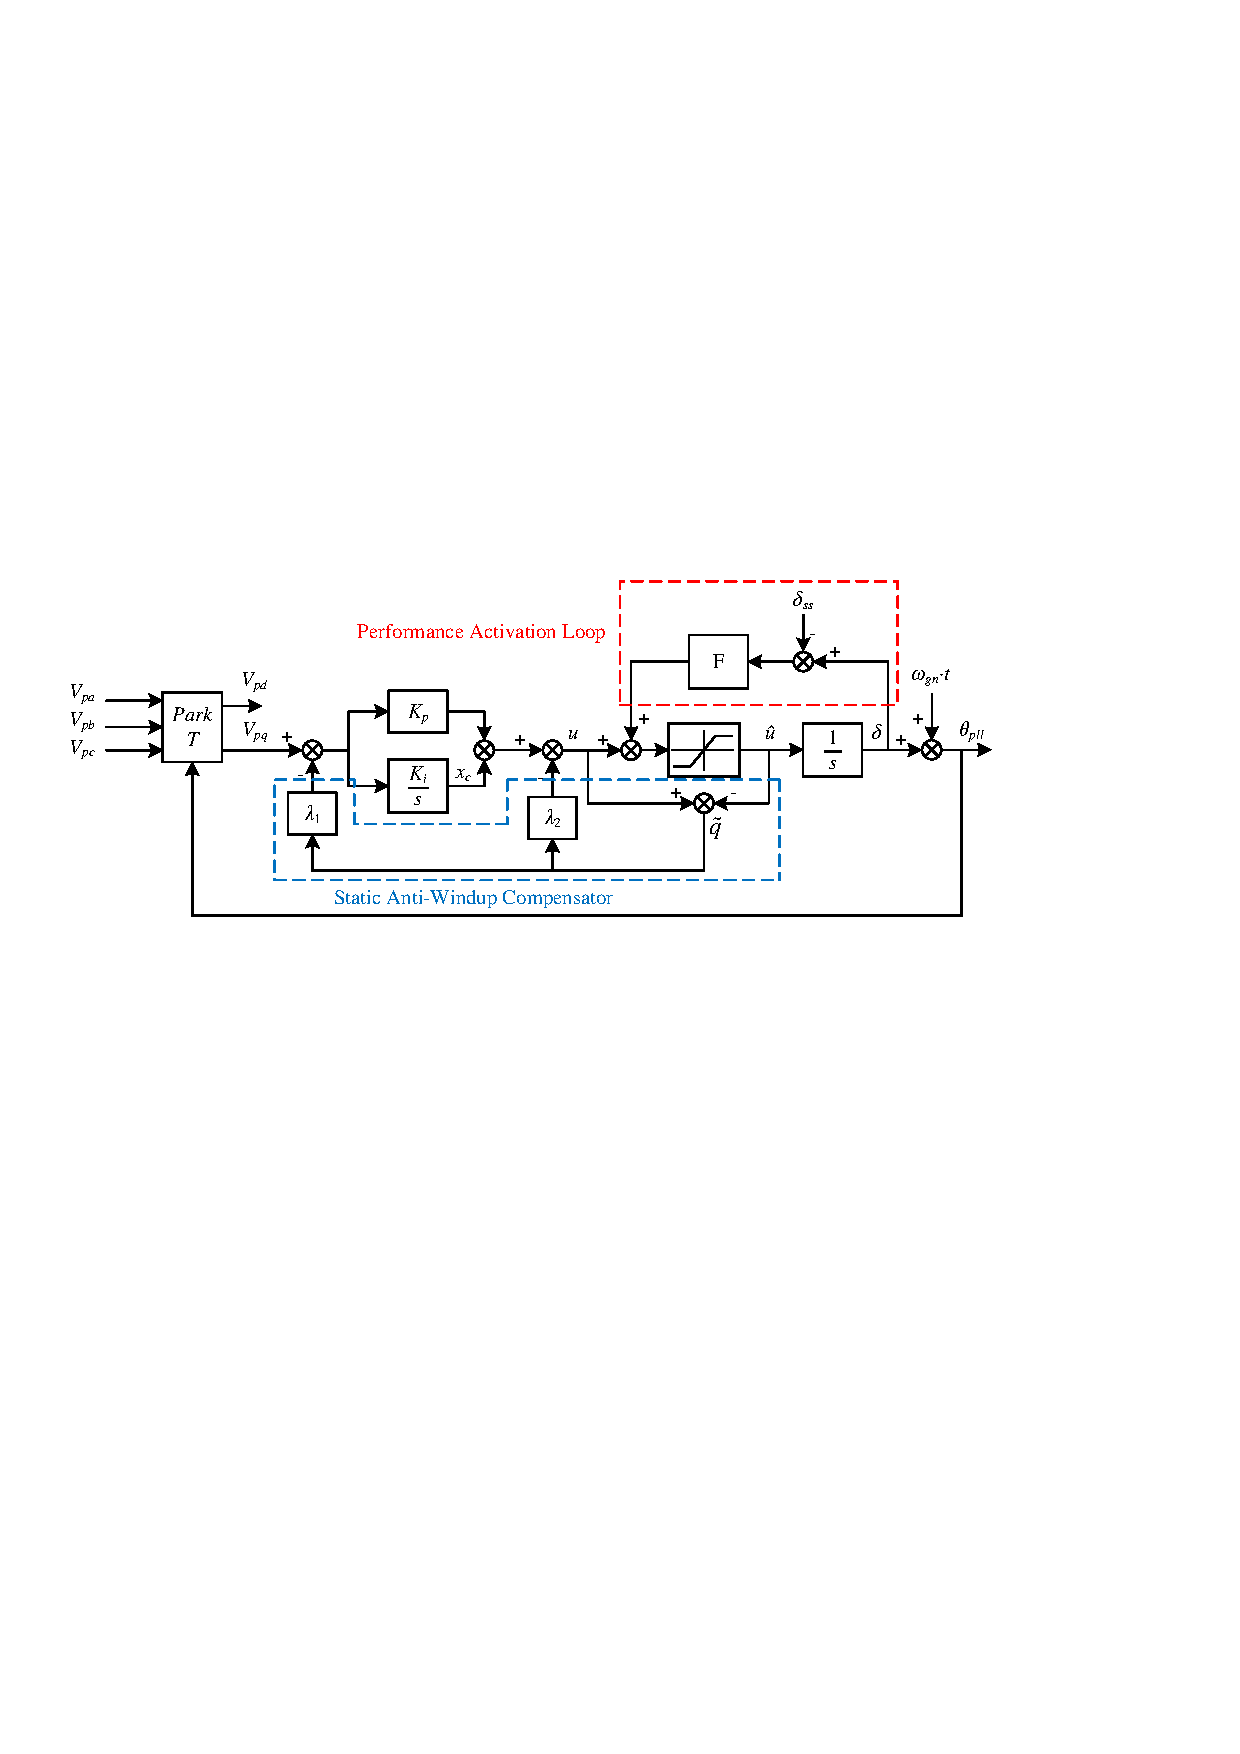
\includegraphics{../Diagrams/PAAWAPLL.pdf}
\caption{Diagram of the performance-activated anti-windup augmented PLL}
\label{fig_paawapll}
\end{figure*}

\subsection{Impact of Grid Fault}
The equilibium points of SRF-PLL exist if and only if $\delta_{ss}$ exists. Moreover, from (\ref{dss}) we know that $\delta_{ss}$ exists if and only if the following condition holds,
\begin{equation}\label{dcond}V_g\geqslant R_gI_q^*+\omega_{gn}L_gI_d^*.\end{equation}

To guarantee the stability of SRF-PLL, its linearized model should be considered. The linearized model of SRF-PLL is given as follows,
\begin{equation}\label{lclSRFPLL}
\bar{\Sigma}_{0}\begin{cases}
    \dot{\bar{x}}=A_{0}\bar{x}+B_{0q}q,\\
    u=C_{0}\bar{x}+D_{0q}q,
\end{cases}
\end{equation}
where $\bar{x}=[\bar{x}_p,\bar{x}_c]^T$ is the state of the linearized model, and
\begin{align*}
A_{0}&=\begin{bmatrix}
    -\dfrac{K_pV_g\cos\delta_{ss}}{C_1}&\dfrac{1}{C_1}\\-\dfrac{K_iV_g\cos\delta_{ss}}{C_1}&\dfrac{K_iL_gI_d^*}{C_1}
\end{bmatrix},&B_{0q}&=\begin{bmatrix}
    -\dfrac{1}{C_1}\\-\dfrac{K_iL_gI_d^*}{C_1}
\end{bmatrix},\\
C_{0}&=\begin{bmatrix}
    -\dfrac{K_pV_g\cos\delta_{ss}}{C_1}&\dfrac{1}{C_1}
\end{bmatrix},&D_{0q}&=-\dfrac{1-C_1}{C_1}.
\end{align*}\par
By analyzing the eigenvalues of $A_{0}$, we obtain the following stablility conditions for SRF-PLL
\begin{align}
    V_g^2&>\left(R_sI_q^*+\omega_{gn}L_gI_d^*\right)^2+\left(\dfrac{42.32L_gI_d^*}{18.4\zeta^2t_s}\right)^2,\label{oscond1}\\
    % \dfrac{18.4L_g}{V_gt_s}&<1.
    V_g&>\frac{18.4L_g}{t_s}.\label{oscond2}
\end{align}\par
From (\ref{dcond}), (\ref{oscond1}) and (\ref{oscond2}), it can be inferred that, with all other conditions being equal, higher $V_g$ means stronger system stability. The grid fault voltage dip
directly reduces $V_g$, thereby harming the system stability.
\subsection{The limitation of the existing anti-windup augmented PLL}
% Saturation nonlinearity does not exist naturally in PLL. In~\cite{tang2023}, an artificial limiter is added after the PI controller in SRF-PLL, resulting in a CPLL, and the simulation
% reveals that the constrained PLL shows stronger transient stability against short-term fault voltage dips than the original SRF-PLL. In~\cite{chen2023}, various trivial anti-windup techniques
% are applied to the constrained PLLs, and the simulation shows that the back-calculation scheme, which is equivalent to a static linear anti-windup compensator, outperforms the other anti-windup
% techniques in short-term FVDT testing. Nevertheless, long-term FVDT is not covered in these researches, which is actually the performance index we cares.\par
The conclusion that a VSC with a CPLL has stronger stability than one with an SRF-PLL stated in~\cite{tang2023} is not well-supported, as the authors only provided some numerical results to support it. According to
existing solid researches on actuator saturation, the artificial limiter added in CPLL would definitely cause the "windup" phenomenon, therefore degrading the stability of the VSC.
Moreover,~\cite{tang2023}~and~\cite{chen2023} only takes short-time grid faults into consideration, with the fault duration being tens to several hundreds of milliseconds. However, most grid faults
cannot be resolved within such a short period, sometimes it even takes several hours to repair the affected area of the grid. Therefore, the system stability under long-term grid faults should be studied.
For grid faults which cause voltage dips, the long-term FVDT, which is the maximum tolerable voltage dip of the specific power system, should be used as the stability index of the VSC.

We obtain the long-term FVDT of VSCs with SRF-PLL, CPLL, and SAWAPLL, respectively, via simulation in two scenarios given in Table~\ref{table_param}. By increasing the fault voltage dip magnitude
$\Delta V_g$ from $0V$ to the value when the fault-time PLL response diverges, we can obtain the FVDT of the VSCs with different PLLs in a specific scenario. The simulation result is shown in Table~\ref{tlim}.
\figurename~\ref{fig_limit} presents an example in the HV scenario. The symbol $f_{pll}$ denotes the grid frequency estimated by the PLL, which is defined as follows
\[f_{pll}=\left\{\begin{aligned}
    &\dfrac{\left(u+\omega_{gn}\right)}{\left(2\pi\right)},\;\textrm{no artificial limiter},\\
    &\dfrac{\left(\hat{u}+\omega_{gn}\right)}{\left(2\pi\right)},\;\textrm{otherwise}.
\end{aligned}\right.\]
\FloatBarrier
\begin{table}[H]
% \renewcommand{\arraystretch}{1.3}
\caption{Long-term FVDT of VSCs with SRF-PLL, CPLL, and SAWAPLL}
\label{tlim}
\centering
\resizebox{\linewidth}{!}{
\begin{tabular}{cccc}
\hline
Scenario & SRF-PLL & CPLL & SAWAPLL\\
\hline
HV & $-63.8\sqrt{2}kV$ & $-62.5\sqrt{2}kV$ & $-66.4\sqrt{2}kV$\\
LV & $-38.9\sqrt{2}V$ & $-37.6\sqrt{2}V$ & $-41.5\sqrt{2}V$\\\hline
\end{tabular}}
\end{table}
It can be inferred from Table~\ref{tlim} that, the artificial limiter added in CPLL actually hurts the synchronization stability of the VSC, which is attributed
to the ``windup'' phenomenon caused by the limiter. The SAWAPLL performs slightly better than the SRF-PLL in long-term FVDT, with a gain of
only around 6 percents. Besides, according to (\ref{dcond}), (\ref{oscond1}) and (\ref{oscond2}), the supremum of the long-term FVDT of a VSC with a SRF-PLL is
$71.762\sqrt{2}kV$ and $44.446\sqrt{2}V$ in the HV and LV scenarios, respectively. These data indicate that the stability improvement achieved by the static
anti-windup compensator is quite limited and falls short of expectations, especially considering the additional computational cost it incurs.

% Section III------------------------------------------------
\section{Performance-Activated Anti-Windup Augmented PLL}\label{sec:paawapll}
\subsection{Modeling}\label{subsec:paawapllm}
Inspired by~\cite{tang2023,chen2023}, based on the work in~\cite{lai2024}, we propose a novel performance-activated anti-windup augmented PLL (PAAWAPLL) which is illustrated in~\figurename~\ref{fig_paawapll}.
% Compared with the conventional SRF-PLL, our design incorporates an artificial limiter to restrain the rate of change of $\delta$, and uses a performance-activated static anti-windup compensator to cope with the "windup" issue caused by the limiter.
Compared with the SAWAPLL, our PAAWAPLL incorporates the error between $\delta_{ss}$ and $\delta$ to the input of the limiter. Since $\delta$ is a signal that can characterize the performance of the PLL, the imported feedback loop allows the system
performance to control the activation timing of the anti-windup compensator. Therefore, by designing an appropriate feedback gain matrix $F$, both transient performance and stability can be enhanced\par
Denote by $\Lambda=[\lambda_1,\lambda_2]^T$ the anti-windup parameters and $F$ the performance-activation gain matrix. Let
\begin{gather*}\hat{u}=\textrm{sat}(u)=\textrm{sgn}(u)\min\left\{|u|,\beta\right\},\\
q=\textrm{dz}(u)=u-\textrm{sat}(u),\end{gather*}
where $\beta$ is the saturation limit. The performance-activated anti-windup augmented PLL is expressed as follows
% \newpage
% \begin{align}\label{paawapll}
% \left\{\begin{aligned}
% \dot{x}_p=&\dfrac{1}{C_1}\left(\left(K_p\lambda_1+\lambda_2+1\right)Fx_p+x_c-K_pV_g\sin\left(x_p+\delta_{ss}\right)\right)\\
%     &+\dfrac{1}{C_1}\left(K_pR_gI_q^*+\left(1-C_1\right)\omega_{gn}-\left(K_p\lambda_1+\lambda_2+1\right)q\right),\\
% \dot{x}_c=&\dfrac{K_i}{C_1}\left(\left(L_gI_d^*\left(\lambda_2+1\right)+\lambda_1\right)Fx_p+L_gI_d^*x_c+R_gI_q^*\right)\\
%     &+\dfrac{K_i}{C_1}\left(-V_g\sin\left(x_p+\delta_{ss}\right)+L_gI_d^*\omega_{gn}\right)\\
%     &+\dfrac{K_i}{C_1}\left(-\left(L_gI_d^*\left(\lambda_2+1\right)+\lambda_1\right)q\right),\\
% u=&\dfrac{1}{C_1}\left(\left(K_p\lambda_1+\lambda_2+1-C_1\right)Fx_p+x_c-K_pV_g\sin\left(x_p+\delta_{ss}\right)\right)\\
%     &+\dfrac{1}{C_1}\left(K_pR_gI_q^*+\left(1-C_1\right)\omega_{gn}-\left(K_p\lambda_1+\lambda_2+1-C_1\right)q\right).
% \end{aligned}\right.
% \end{align}
\begin{equation}\label{paawapllm}
\left\{\begin{aligned}
    \dot{x}=&\left(\left(A_p\Lambda+A_c\right)FI_1+A_cI_2\right)x-\left(A_p\Lambda+A_c\right)q+d,\\
    u=&\left(\left(C_p\Lambda+C_c-1\right)FI_1+C_cI_2\right)x\\
    &-\left(C_p\Lambda+C_c-1\right)q+I_1d,
\end{aligned}\right.
\end{equation}
where
\begin{align*}A_p&=\begin{bmatrix}
    \dfrac{K_p}{C_1}&\dfrac{1}{C_1}\\\dfrac{K_i}{C_1}&\dfrac{K_iL_gI_d^*}{C_1}
\end{bmatrix},\;A_c=\begin{bmatrix}
    \dfrac{1}{C_1}\\\dfrac{K_iL_gI_d^*}{C_1}
\end{bmatrix},\\
C_p&=I_1A_p,\;C_c=I_1A_c,\;I_1=\begin{bmatrix}
    1&0
\end{bmatrix},\;I_2=\begin{bmatrix}
    0&1
\end{bmatrix},\\
d&=\begin{bmatrix}
    \dfrac{K_p}{C_1}\\
    \dfrac{K_i}{C_1}
\end{bmatrix}\left(R_gI_q^*+L_gI_d^*\omega_{gn}-V_g\sin\left(x_p+\delta_{ss}\right)\right).\end{align*}

Since the sine terms are bounded, $d$ can be viewed as an origin-passing perturbation.

Because of the existence of the algebraic loop
\begin{multline}\label{algloop}
u+\left(C_{p1}-1\right)\left(u-sat(u)\right)=\left(\left(C_{p1}-1\right)FI_1+C_cI_2\right)x
\end{multline}
in (\ref{paawapllm}), the well-posedness, i.e., the existence and uniqueness of the solution $u$, must be guaranteed. One sufficient well-posedness condition of the algebraic
loop (\ref{algloop}) is that there exists a diagonal matrix $W>0$ satisfying
\begin{equation}\label{wpcond}
    -\textrm{He}\left(C_{p1}^TW\right)-2W<0.
\end{equation}\par

\subsection{Anti-Windup Synthesis}\label{subsec:awsyn}
\begin{figure}[!t]
\centering
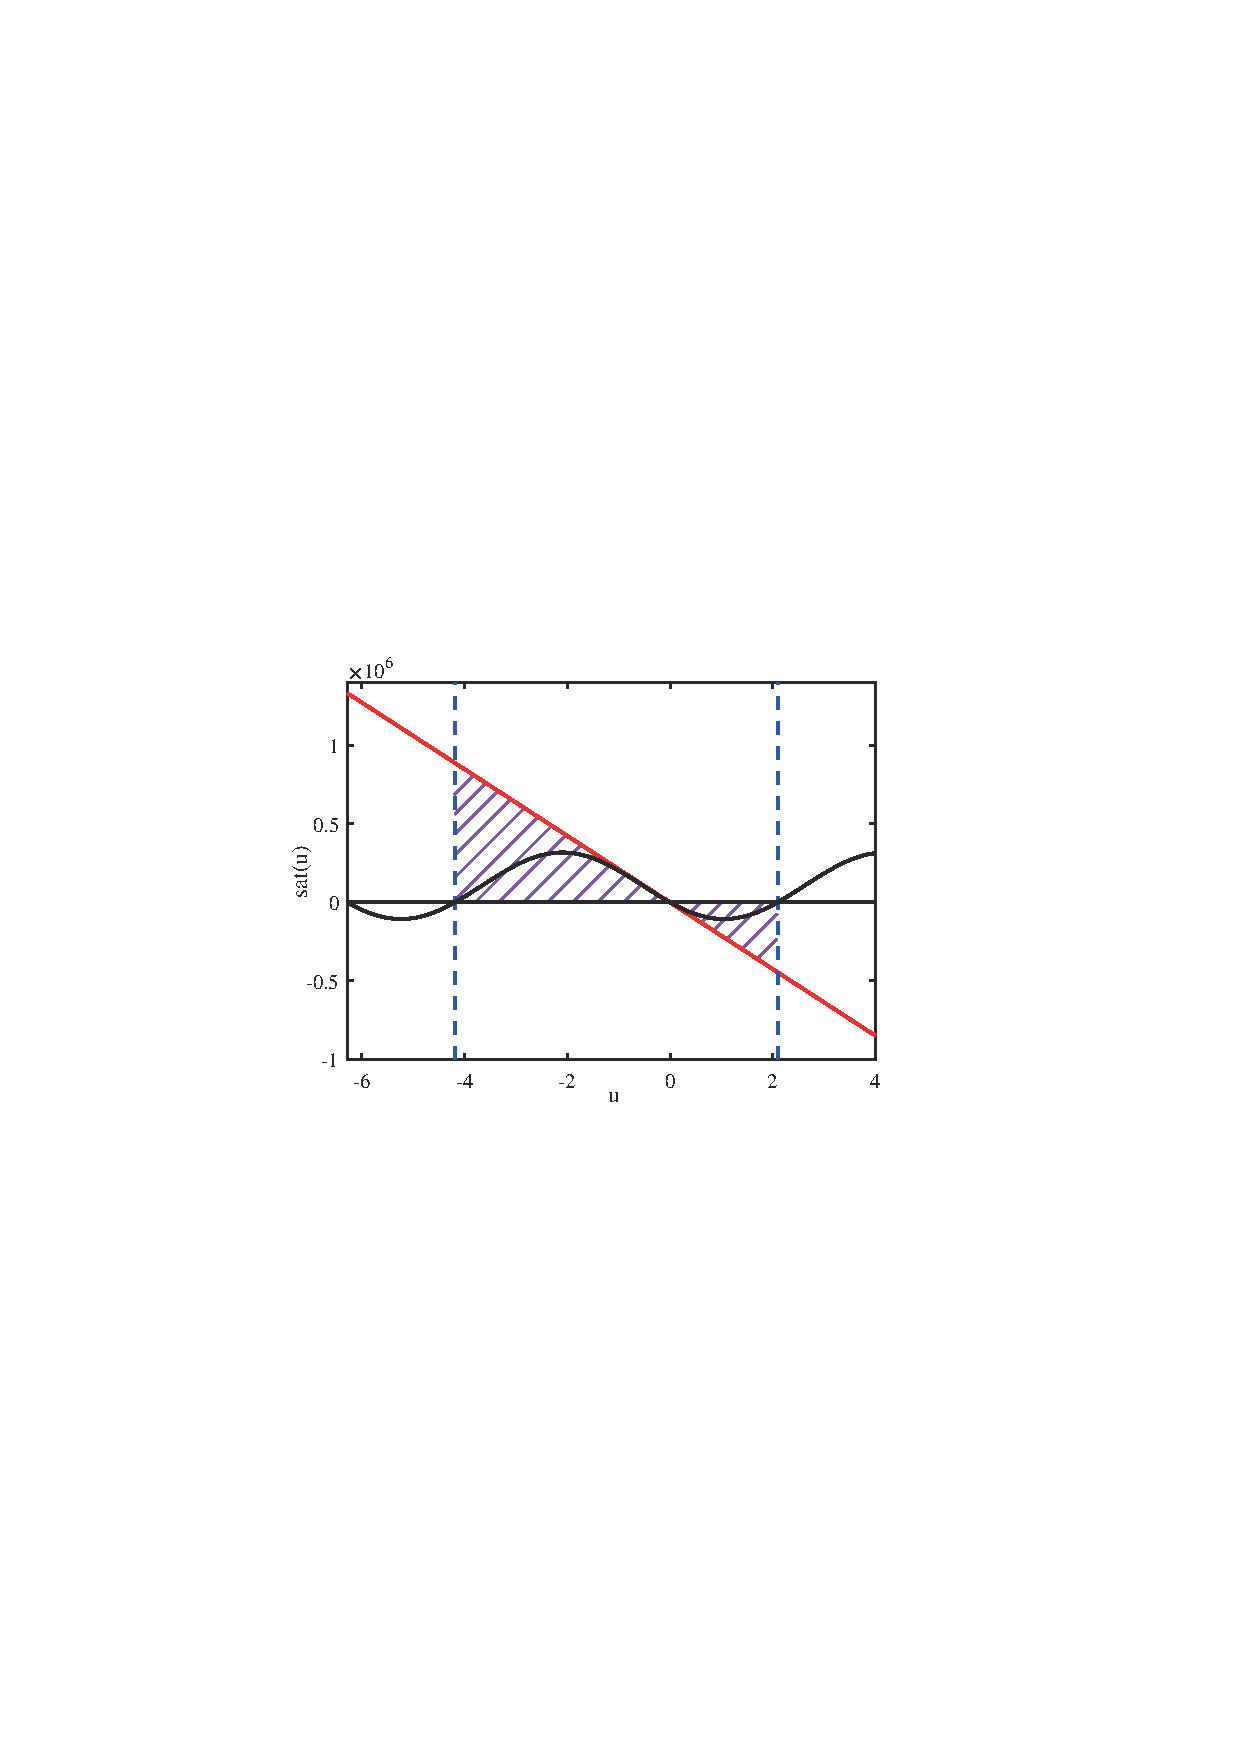
\includegraphics[width=1.0\linewidth]{../Diagrams/convexhull.pdf}
\caption{Diagram of regional convex hull}
\label{fig_conv}
\end{figure}
The aim of anti-windup synthesis is to develop a compensator that reduces the impact of saturation on performance and stability. This requires formulating
an optimization problem that maximizes the system $R_A$ while ensuring that the stability criteria are met.\par
Anti-windup synthesis for general nonlinear systems with saturation remains a challenging and unresolved issue, with only a few methods available for some
specific nonlinear systems\cite{wen2011,hermann2010,yong2020}. Since the stability of a nonlinear system's equilibrium point can be determined by the stability
of its linearized counterpart\cite{bookofkhalil}, we apply the anti-windup synthesis result of the linearized system to the original nonlinear system (\ref{paawapllm}).
% focuses on anti-windup synthesis for the linearized system~(\ref{paawapllm}) around the origin.
% The objective of anti-windup synthesis is to design a compensator such that the performance and stability degradation caused by saturation is minimized.
% To achieve this, we need to form an optimization problem which maximizes the system $R_A$ and meets the stability and performance constraints.
% The anti-windup synthesis for generic nonlinear systems with saturation still remains an open problem, and only a few methods for some specific
% nonlinear systems have been proposed\cite{wen2011,hermann2010,yong2020}. Since the stability of an equilibrium point of a nonlinear system can be
% concluded from the stability of the equilibrium point of its linearization\cite{bookofkhalil}, in this paper, the anti-windup synthesis is performed on the
% linearized system~(\ref{paawapllm}) around the origin.
% For a linear system with bounded control, a state $x_0$ is said to be null controllable in time $T>0$ if there exists a bounded control $u$ such
% that the state trajectory $x(t)$ of the system satisfies $x(0)=x_0$ and $x(T)=0$. The set of all null controllable states in some time $T\in[0,+\infty)$ is called
% the null controllable region at time $T$, which is denoted by $\mathcal{C}(T)$. In further, denote by $mathcal{C}$ the set of all null controllable states,
% then it is easy to find out that $\mathcal{C}=\cup_{T\in[0,+\infty)}\mathcal{C}(T)$.

Given a system $\dot{x}=f(x),x\in\mathbb{R}^n$ and an initial condition $x(0)=x_0$, we define the state trajectory as $\phi(t,x_0)$. Suppose the origin is an equilibrium point of
the system, and then its $R_A$ can be defined as 
% For a system $\dot{x}=f(x)$, where $x\in\mathbb{R}^n$, given an initial state $x(0)=x_0$, denote the trajectory of the system as $\phi(t,x_0)$. Then, the $R_A$ of the origin is defined as
\[R_A:=\{x_0\in\mathbb{R}^n:\lim_{t\rightarrow+\infty}\phi(t,x_0)=0\}.\]\par
% Obviously, $R_A\subseteq\mathcal{C}$.
In general, it is not feasible to determine the exact $R_A$ of a linear system with saturation feedback. Nevertheless, for a planar system with a single input, its boundary of $R_A$ corresponds to its unique
convex limit cycle\cite{alvarez1993,bookofhu,bookofli}. This characteristic allows us to approximate $R_A$ using certain tractable sets.
% It is in general impossible to determine the $R_A$ of a linear system with saturation feedback. However, for a planar system with a single input, the boundary of $R_A$ is the unique convex limit
% cycle of the system\cite{alvarez1993,bookofhu,bookofli}. This enables us to approximate $R_A$ using some approachable sets.

The invariant set is a logical choice for approximating $R_A$. It is defined as a set that all state trajectories originating within it stay within it. Moreover, if these trajectories
tend to converge towards an equilibrium point within the set, it is considered a contractively invariant set, which makes it a valid estimate of $R_A$.
% Invariant set is a natural candidate for estimation of $R_A$. A set is called an invariant set of the system if all state trajectories starting
% from it remains inside it. Futhermore, if these trajectories converge to an equilibrium point inside the set,then the set is a contractively invariant set and is an estimate of $R_A$.

Ellipsoidal invariant sets has been widely used as the level sets of Lyapunov functions in estimating $R_A$ for high-order systems and nonlinear systems, due to its simplicity\cite{silva2005,bookofhu,hu2002}. Define a quadratic Lyapunov
function as $V(x)=x^TPx$, where $P\in\mathbb{R}^{n\times n}$ is positive-definite. For a given positive number $\rho$, the ellipsoidal level set is defined as $\mathcal{E}(P,\rho)=\{x\in\mathbb{R}^n:x^TPx\leqslant\rho\}$.
Then, Definition~\ref{condcis} provides the criteria under which $\mathcal{E}(P,\rho)$ qualifies as a contractively invariant set of the system.
% Because of its simple form as a level set of a quadratic Lyapunov function, ellipsoidal invariant set has been widely used in estimating the region of attraction for high order systems and nonlinear systems\cite{silva2005,bookofhu,hu2002}.
% Construct a quadratic Lyapunov function $V(x)=x^TPx$, where $P\in\mathbb{R}^{n\times n}$ is positive-definite. Given a positive real number $\rho$, define the ellipsoidal level set
% as $\mathcal{E}(P,\rho)=\{x\in\mathbb{R}^n:x^TPx\leqslant\rho\}$, then Definition~\ref{condcis} gives the condition for $\mathcal{E}(P,\rho)$ to be contractively invariant.
\begin{definition}\label{condcis}
$\mathcal{E}(P,\rho)$ is a contractively invariant set of the system $\dot{x}=f(x)$, if
\[\dot{V}(x)=2x^TPf(x)<0,\]
holds for any $x\in\mathcal{E}(P,\rho)\setminus\{0\}$.
\end{definition}

Let $A_{p1}=A_p\Lambda+A_c$, then the following contractive invariance condition for $\mathcal{E}(P,\rho)$ can be obtained from Definition~\ref{condcis}.
\begin{equation}\label{lyapf}
\dot{V}=2x^TP\left(A_{p1}FI_1+A_cI_2\right)x+2x^TP\left(-A_{p1}q+d\right)<0.
\end{equation}

Besides, the following condition needs to be satisfied to ensure that there exists $\rho$ for $\mathcal{E}(P,\rho)$ to be contractively invariant.
\begin{equation}\label{olcond}\mathrm{He}\left(PA_{p1}FI_1+PA_cI_2\right)<0.\end{equation}

Because of the existence of nonlinearities $q$ and $d$, (\ref{lyapf}) cannot be solved directly. These nonlinearities must be eliminated from the inequalities to make them feasible.
First, we deal with $d$. Note that $d$ is periodic and origin-crossing. Thus we can use the following regional convex hull to handle it,%~\figurename~\ref{fig_conv} illustrates the regional convex hull.
\begin{equation}\label{localch}
    d\in\mathrm{co}\{0,Lx\},\;\forall x\in D_x,
\end{equation}
where
\begin{gather*}
L=\begin{bmatrix}
    -\dfrac{K_pV_g}{C_1}&0\\-\dfrac{K_iV_g}{C_1}&0
\end{bmatrix},\\
D_x=\{x:I_1x\in[-\pi-2\delta_{ss},\pi-2\delta_{ss}]\}.
\end{gather*}\par
The geometric imterpretation of the regional convex hull is depicted in~\figurename~\ref{fig_conv}.\par
Then we obtain the following differential inclusion
\begin{align}\label{diffinclu}
    &\dot{x}\in\mathcal{F}(x,q,\eta)\\
    &\;\:=\mathrm{co}\left\{\begin{gathered}\left(A_{p1}FI_1+A_cI_2\right)x-A_{p1}q ,\\
    \left(A_{p1}FI_1+A_cI_2+L\right)x-A_{p1}q\end{gathered}\right\}.\notag
\end{align}\par
Thus, for any $x\in\mathcal{E}(P,\rho)\subseteq D_x$, there exists a scalar $\eta\in[0,1]$, such that
\begin{equation}
\dot{x}=\left(A_{p1}FI_1+A_cI_2+\eta L\right)x-A_{p1}q,
\end{equation}
and (\ref{lyapf}) can be reevaluated as
\begin{equation}\label{convhlyapf}
    \dot{V}=2x^TP\left(A_{p1}FI_1+A_cI_2+\eta L\right)x-2x^TPA_{p1}q<0.
\end{equation}\par
An obvious sufficient condition for (\ref{convhlyapf}) to hold is shown below
\begin{gather}
    \label{vt1lyapf}\dot{V}_1=2x^TP\left(A_{p1}FI_1+A_cI_2\right)x-2x^TPA_{p1}q<0,\\
    \label{vt2lyapf}\dot{V}_2=2x^TP\left(A_{p1}FI_1+A_cI_2+L\right)x-2x^TPA_{p1}q<0.
\end{gather}\par
Now that the disturbance $d$ has been handled, the next step is to addresss the deadzone $q$.\par
Regional sector condition is the traditional way of dealing with saturation or deadzone nonlinearities\cite{bookofzac,bookofli}.
Suppose that the input of saturation is $u\in\mathbb{R}^m$, given a matrix $H\in\mathbb{R}^{m\times n}$, define
\[\mathcal{L}(H)=\{x\in\mathbb{R}^n:|Hx|_{\infty}\leqslant\beta\}.\]
$\mathcal{L}(H)$ is the linear zone of $\mathrm{sat}(Hx)$. Then, lemma~\ref{lemma} gives a definition of
the regional sector condition.
\begin{lemma}\label{lemma}
For any $x\in\mathcal{L}(H)$ and diagonal matrix $W\in\mathbb{R}^{n\times n}$ which is positive-definite, the following two equivalent
inequalities hold
\begin{gather*}
(u-\mathrm{sat}(u))^TW(\mathrm{sat}(u)+Hx)\geqslant0,\\
q^TW(u-q+Hx)\geqslant0.
\end{gather*}
\end{lemma}\par
By adding the regional sector condion to the contractive invariance condition of $\mathcal{E}(P,\rho)$, an linear quadratic inequality can be formed,
where $x$ and $q$ are the free variables, therefore the deadzone $q$ is eliminated in the solving procedure.\par
% Let $C_{p1}=C_p\Lambda+C_c$, then the following regional sector condition holds for any $x\,\mathrm{s.t.}\,\mathrm{sat}(Hx)=Hx$
% % we apply the following traditional regional sector condition to cope with the deadzone $q$.
% \begin{multline}\label{seccond}
% q^TW\left(\left(C_{p1}FI_1+C_cI_2+H\right)x-C_{p1}q\right)\geqslant 0,\\
% \forall x\;\mathrm{s.t.}\;\mathrm{sat}(Hx)=Hx,
% \end{multline}
The regional sector condition of the corresponding system of (\ref{vt1lyapf}) is
\begin{equation}\label{seccond}
q^TW\left(\left(C_{p1}FI_1+C_cI_2+H\right)x-C_{p1}q\right)\geqslant 0,\forall x\in\mathcal{L}(H).
\end{equation}
Then, add (\ref{seccond}) to (\ref{vt1lyapf}) so that we get the following sufficient condition for (\ref{vt1lyapf}) to hold
% modified condition for $\mathcal{E}(P,\rho)$ to be a contractively invariant set of the corresponding system of (\ref{vt1lyapf})
\begin{equation}\label{stbcond}
    \dot{V}_1\leqslant\dot{V}_1+2q^TW\left(C_{p1}FI_1+C_cI_2+H\right)x-2q^TWC_{p1}q<0,
\end{equation}
which is equivalent to
\begin{equation}\label{awbmiv1}
\mathrm{He}\begin{bmatrix}
    PA_{cl}&-P(A_p\Lambda+A_c)\\
    W\left(I_1A_{cl}+H\right)&-W\left(C_p\Lambda+C_c\right)
\end{bmatrix}<0,
\end{equation}
where $A_{cl}=A_{p1}FI_1+A_cI_2$. The deadzone $q$ becomes a free variable and thus is eliminated in the matrix inequality (\ref{awbmiv1}).\par
In the same way, the sufficient condition for (\ref{vt2lyapf}) to hold can obtained as follows
\begin{equation}\label{awbmiv2}
\mathrm{He}\begin{bmatrix}
    P\left(A_{cl}+L\right)&-P(A_p\Lambda+A_c)\\
    W\left(I_1A_{cl}+I_1L+H\right)&-W\left(C_p\Lambda+C_c\right)
\end{bmatrix}<0.
\end{equation}\par
Additionally, to ensure that the regional sector condition holds for any $x\in\mathcal{E}(P,\rho)$, the following condition should hold, which is,
\begin{equation}\label{seclmi}
\!\!\!\!\!\!\!\!\mathcal{E}(P,\rho)\subseteq\mathcal{L}(H)\Longleftrightarrow
\begin{bmatrix}
    P&H^T\\H&\beta^2/\rho
\end{bmatrix}\geqslant0.
\end{equation}\par
The combination of (\ref{awbmiv1}), (\ref{awbmiv2}) and (\ref{seclmi}) yields a sufficient condition for $\mathcal{E}(P,\rho)$ to be a contractively invariant
set of the system (\ref{paawapllm}).\par
% Besides, to ensure that the sector condition holds in $\epsilon\left(P\right)$, it should hold that
% %To ensure that all points in $\mathcal{E}(P)$ satisfies (\ref{seccond}),
% \[\dfrac{x^TH^THx}{\beta^2}\leqslant x^TPx\]
% i.e.
% \begin{equation}\label{seclmi}
% \begin{bmatrix}
%     P&H^T\\H&\beta^2
% \end{bmatrix}\geqslant0
% \end{equation}\par
Both (\ref{olcond}) and (\ref{wpcond}) are already incorporated in (\ref{awbmiv1}) and (\ref{awbmiv2}).\par
% Now we have obtained all the essential constraints to form an optimization problem for solving parameters of the anti-windup compensator, and the last thing is to determine the objective function which should be an index of the
% size of $R_A$.
For optimization objective, we simply choose $-\rho$ as the objective function, since $\rho$ directly represents the size of $\mathcal{E}(P,\rho)$.

Finally, an optimization problem maximizing the size of the contractively invariant set $\mathcal{E}(P,\rho)$ is formulated below
\begin{flalign}
&\ \label{optimnc}\begin{array}{cc}\mathop{\min.}\limits_{\rho>0,P>0,W>0,F,\Lambda,H}&-\rho\end{array} &\\
&\ \begin{array}{cl}
    \textrm{s.t.}&\textrm{inequalities}\;(\ref{awbmiv1}),(\ref{awbmiv2}),(\ref{seclmi}).
\end{array}\notag &
\end{flalign}\par
% To determine the anti-windup parameters $\Lambda$ and $F$ which maximize $\epsilon(P)$, following the polyhedron method presented in~\cite{silva2005}, we define a polyhedron $\Xi$ as:
% \[\Xi=\mathbf{conv}\{v_1,\cdots,v_{n_{r}}\},v_r\in\mathbb{R}^2,r\in I[1,n_r]\]
% then maximizing $\epsilon(P)$ is equivalent to maximizing $\gamma$. The condition that $\gamma\Xi\subset\mathcal{E}(P)$ could be written as:
% \begin{equation}\begin{bmatrix}\label{phlmi}
%     \dfrac{1}{\gamma^2}&v_r^T\\v_r&P^{-1}
% \end{bmatrix}\geqslant0,\quad r\in I[1,n_r]\end{equation}
However, the optimization problem (\ref{optimnc}) is not convex, as non-convex terms like $\Lambda F$ appears in the constraints. To eliminate the non-convex terms in (\ref{optimnc}),
some nonlinear transformation needs to be performed\cite{bookofzac}. Let $Q=P^{-1},U=W^{-1},Y=HQ$, then the following optimization problem can be obtained
% The cross terms in (\ref{awbmiv1}) and (\ref{awbmiv2}) makes it impossible to solve out $\Lambda, F$ simultaneously. We address this problem by importing a nonlinear transformation and
% developing an iterative optimization algorithm.
\begin{flalign}
&\ \label{optimc}\begin{array}{cc}\mathop{\min.}\limits_{\rho>0,Q>0,F,U>0,\Lambda,Y}&-\rho\end{array} &\\
&\ \begin{array}{cl}
    \textrm{s.t.}&\mathrm{He}\begin{bmatrix}
        A_{cl}Q&-(A_p\Lambda+A_c)U\\\left(I_1A_{cl}+H\right)Q&-\left(C_p\Lambda+C_c\right)U
    \end{bmatrix}<0,\\
    &\mathrm{He}\begin{bmatrix}
        \left(A_{cl}+L\right)Q&-(A_p\Lambda+A_c)U\\\left(I_1A_{cl}+I_1L+H\right)Q&-\left(C_p\Lambda+C_c\right)U
    \end{bmatrix}<0,\\
    % &\begin{bmatrix}
    %     \mu&v_i^T\\v_i&Q
    % \end{bmatrix}\geqslant0,\forall i\in I[1,n_r]\\
    &\begin{bmatrix}
        Q&Y^T\\Y&\beta^2/\rho
    \end{bmatrix}\geqslant0.
\end{array}\notag &
\end{flalign}\par
\begin{table*}
% \renewcommand{\arraystretch}{1.3}
\caption{Circuit and controller parameters in simulation}
\label{table_param}
\centering
\tabcolsep=.05\linewidth
\renewcommand{\arraystretch}{1.2}
% \resizebox{\linewidth}{!}{
\begin{tabular}{cccc}
\hline
Symbol & Description & HV Scenario & LV Scenario\\
\hline
$V_{g}$ & Magnitude of the grid voltage & $150\sqrt{2}kV$ & $100\sqrt{2}V$\\
$\omega_{gn}$ & Nominal grid angular frequency & $100\pi$ & $100\pi$\\
$I_d^*$ & {\makecell[c]{Magnitude of d-axis\\current reference of VSC}} & $1kA$ & $20A$\\
$I_q^*$ & {\makecell[c]{Magnitude of q-axis\\current reference of VSC}} & $0A$ & $0A$\\
$R_f$ & {\makecell[c]{Resistance of the VSC\\output low-pass filter}} & $0\Omega$ & $0\Omega$\\
$L_f$ & {\makecell[c]{Inductance of the VSC\\output low-pass filter}} & $15mH$ & $1.5mH$\\
$R_g$ & Grid resistance & $106\Omega$ & $3.75\Omega$\\
$L_g$ & Grid inductance & $338mH$ & $12mH$\\
$\zeta$ & {\makecell[c]{Damping ratio in\\PLL parameter design}} & $0.5$ & $0.5$\\
$t_s$ & {\makecell[c]{Settling time in\\PLL parameter design}} & $0.1s$ & $0.1s$\\
$\beta$ & Saturation limit & $10\pi$ & $10\pi$\\
$\Lambda$ & Anti-windup parameters & $\begin{bmatrix}517.14,-1.3917\end{bmatrix}^T$ & $\begin{bmatrix}5.9289,-7.7758\end{bmatrix}^T$\\
$F$ & Performance-activation gain & $-348.11$ & $-208.55$\\\hline
\end{tabular}
% }
\end{table*}
Then the following iterative algorithm can be developed.\\
\textbf{Algorithm 1}\\
\textbf{Step 1:} Fix $F=0$, let $Z=\Lambda U$, solve the optimization prpblem (\ref{optimnc}) to obtain $\Lambda=ZU^{-1}$\\
\textbf{Step 2:} Choose an initial value $F_1$ for $F$, threshold $\alpha$ and the maximum iteration number $k_m$. Let $k=1$.\\
\textbf{Step 3:} Fix $\Lambda, F_k$, solve the optimization problem (\ref{optimnc}). Denote by $\left(\tilde{\rho},\tilde{Q},\tilde{U},\tilde{Y}\right)$ the solution. Let $\rho_k=\tilde{\rho}$, update $Q$ with $\tilde{Q}$.\\
\textbf{Step 4:} If $k\geq2$ and $|\rho_k-\rho_{k-1}|<\alpha$, then stop, and take $\Lambda, F_k$ as outputs; else, if $k=k_m$, then stop, and select the minimum $\rho_t$ among all $\rho_k$, and take $\Lambda, F_t$ as outputs;
else, let $k=k+1$, go to step 5.\\
\textbf{Step 5:} Fix $\Lambda, Q$, solve the optimizatioon problem (\ref{optimnc}). Denote by $\left(\tilde{\rho},\tilde{F},\tilde{U},\tilde{Y}\right)$ the solution. Let $F_k=\tilde{F}$. Go back to step 3.

% Section IV------------------------------------------------

\section{Validation}\label{sec:valid}
% \subsection{Simulation Results}
To illustrate the effectiveness of the PAAWAPLL in improving the synchronization stability of RES-VSC, we carry out simulations in two different scenarios, one is the low-voltage (LV) scenario, and the other
is the high-voltage (HV) scenario. The circuit and controller parameters of the two scenarios are listed in Table~\ref{table_param}. In each scenario, we test the responses of VSCs with SRF-PLL, CPLL, SAWAPLL, and
PAAWAPLL, respectively, under several fault conditions, for obtaining the long-term FVDT of them. The system is said to be able to tolerate a specific fault voltage dip if the fault-time $x_p$ always falls
in the range $(-\pi-2\delta_{ss},\pi-2\delta_{ss})$ and converges to $0$ once the fault is resolved.
% \FloatBarrier
\begin{table}[H]
% \renewcommand{\arraystretch}{1.3}
\caption{long-term FVDT of VSCs with SRF-PLL, CPLL, SAWAPLL and PAAWAPLL}
\label{tlf}
\centering
\resizebox{\linewidth}{!}{
\begin{tabular}{ccccc}
\hline
Scenario & SRF-PLL & CPLL & SAWAPLL & PAAWAPLL\\
\hline
HV & $-63.8\sqrt{2}kV$ & $-62.5\sqrt{2}kV$ & $-66.4\sqrt{2}kV$ & $-149.9\sqrt{2}kV$\\
LV & $-38.9\sqrt{2}V$  & $-37.6\sqrt{2}V$  & $-41.5\sqrt{2}V$  & $-99.9\sqrt{2}V$\\\hline
\end{tabular}}
\end{table}
The long-term FVDT of VSCs with the four PLLs is shown in Table \ref{tlf}, from which it can be infered that the PAAWAPLL dramatically improves the long-term FVDT of the grid-following VSC.
% In each scenario, we record the transient responses of the unconstrained, the static anti-windup augmented and our proposed PLLs under two different fault conditions. The fault conditions are listed in Table~\ref{table_fault}.
% In both scenarios, there is no equilibrium point existing during fault. The system configuration follows~\figurename~\ref{fig_vsc}, with the VSC being modeled by a controlled voltage source.
Figs.~\ref{fig_HVsim} and \ref{fig_LVsim} present some simulation results in the HV and LV scenarios, respectively.\par
\begin{figure*}[!t]
\centering
\subfloat[][]{
\includegraphics[width=.5\linewidth]{../Diagrams/simulation_results_j/HVf2.pdf}}
\subfloat[][]{
\includegraphics[width=.5\linewidth]{../Diagrams/simulation_results_j/HVf3.pdf}}
\caption{Simulation result of VSCs with SRF-PLL, CPLL, SAWAPLL, and PAAWAPLL, in the HV scenario. The fault voltage dip magnitude is $-66\sqrt{2}kV$ in (a) and $-149\sqrt{2}kV$ in (b).}
\label{fig_HVsim}
\end{figure*}
\begin{figure*}[!t]
\centering
\subfloat[][]{
\includegraphics[width=.5\linewidth]{../Diagrams/simulation_results_j/LVf2.pdf}}
\subfloat[][]{
\includegraphics[width=.5\linewidth]{../Diagrams/simulation_results_j/LVf3.pdf}}
\caption{Simulation result of VSCs with SRF-PLL, CPLL, SAWAPLL, and PAAWAPLL, in the LV scenario. The fault voltage dip magnitude is $-41\sqrt{2}V$ in (a) and $-99\sqrt{2}V$ in (b).}
\label{fig_LVsim}
\end{figure*}
The simulation outcome is a sufficient and compelling evidence to demonstrate the efffectiveness of the proposed PLL configuration.
% \subsection{Experiment Results}
% Remaining unfinished.
% Section V------------------------------------------------
\section{Conclusion}\label{sec:conclusion}
In this paper, a novel PLL configuration with performance-activated anti-windup compensation is proposed for improving the synchronization stability of grid-following VSC under severe grid faults. Detailed PLL
parameter determination and anti-windup synthesis methodology is elaborated. Simulation results show the significant synchronization stability enhancement achieved by the proposed PLL configuration in comparison
with the original SRF-PLL and some other existing PLL configurations.

% \balance

\bibliographystyle{IEEEtran}
\bibliography{IEEEabrv, references}

%\begin{IEEEbiography}[{\includegraphics[width=1in,height=1.25in,clip,keepaspectratio]{fig1.png}}]{IEEE Publications Technology Team}
%In this paragraph you can place your educational, professional background and research and other interests.\end{IEEEbiography}

\end{document}